
%(BEGIN_QUESTION)
% Copyright 2011, Tony R. Kuphaldt, released under the Creative Commons Attribution License (v 1.0)
% This means you may do almost anything with this work of mine, so long as you give me proper credit

Examine this {\it valve signature} taken from a valve that clearly has problems, and answer the questions that follow:

$$\includegraphics[width=15.5cm]{i00426x01.eps}$$

\begin{itemize}
\item{} Is this an air-to-open valve, or an air-to-close valve? 
\vskip 10pt
\item{} Which axis of the graph (horizontal or vertical) represents (percent of) valve stem position?
\vskip 10pt
\item{} Which axis of the graph (horizontal or vertical) represents (percent of) actuator air pressure?
\vskip 10pt
\item{} What kind of problem does this valve have, and how might it be fixed?
\end{itemize}

\underbar{file i00426}
%(END_QUESTION)




%(BEGIN_ANSWER)

\noindent
{\bf Partial answer:}

\begin{itemize}
\item{} Is this an air-to-open valve, or an air-to-close valve? {\it It is air-to-close.  We know this from the negative slope of the traces: more air pressure is required to move the valve stem further closed.}
\vskip 10pt
\item{} Which axis of the graph (horizontal or vertical) represents (percent of) valve stem position? {\it The horizontal axis.  We can tell this by the steep ``down'' and ``up'' turns at each end of the plots: here actuator pressure spikes with little or no motion of the stem because the stem has reached its mechanical limit.}
\end{itemize}

%(END_ANSWER)





%(BEGIN_NOTES)

\begin{itemize}
\item{} Is this an air-to-open valve, or an air-to-close valve? {\it It is air-to-close.  We know this from the negative slope of the traces: more air pressure is required to move the valve stem further closed.}
\vskip 10pt
\item{} Which axis of the graph (horizontal or vertical) represents (percent of) valve stem position? {\it The horizontal axis.  We can tell this by the steep ``down'' and ``up'' turns at each end of the plots: here actuator pressure spikes with little or no motion of the stem because the stem has reached its mechanical limit.}
\vskip 10pt
\item{} Which axis of the graph (horizontal or vertical) represents (percent of) actuator air pressure? {\it The vertical axis, for the same reason as above.}
\vskip 10pt
\item{} What kind of problem does this valve have, and how might it be fixed? {\it There is an incredible amount of friction in the valve mechanism toward the closed (seated) position.  Either the trim is mechanically damaged or it was improperly assembled.}
\end{itemize}

%INDEX% Final Control Elements, valve: diagnostic signature for pneumatic actuator

%(END_NOTES)


